\documentclass[11pt]{amsart}
\usepackage[margin=1.15in]{geometry}
\usepackage{amssymb,amsmath,mathtools}
\usepackage{graphicx,booktabs,array,float}
\usepackage[section]{placeins}
\usepackage[hidelinks]{hyperref}
\usepackage[expansion=false]{microtype}

\newtheorem{theorem}{Theorem}[section]
\newtheorem{proposition}[theorem]{Proposition}
\newtheorem{lemma}[theorem]{Lemma}
\newtheorem{corollary}[theorem]{Corollary}
\newtheorem{mainthm}{Theorem}
\renewcommand{\themainthm}{\Alph{mainthm}}
\theoremstyle{definition}
\newtheorem{definition}[theorem]{Definition}
\newtheorem{remark}[theorem]{Remark}
\newtheorem{example}[theorem]{Example}

\newcommand{\ZZ}{\mathbb{Z}}
\newcommand{\QQ}{\mathbb{Q}}
\newcommand{\CC}{\mathbb{C}}
\newcommand{\HH}{\mathbb{H}}
\newcommand{\e}{\mathbf e}
\newcommand{\vt}{\vartheta}
\newcommand{\cH}{\mathcal H}
\newcommand{\coef}[2]{\big[#2\big]#1}
\newcommand{\zenodoDOI}{10.5281/zenodo.XXXXXXXX}

\setlength{\emergencystretch}{2.5em}
\hbadness=2000
\raggedbottom
\begin{document}

\title[Black holes carry positive discrete information]{Black Holes Carry Positive\\ Discrete Information}

\author{Deep Bhattacharjee}
\address{Formerly, Electro-Gravitational Space Propulsion Laboratory (EGSPL), Bhubaneswar, Odisha 751030, India}
\address{Formerly, University of Calcutta (Heramba Chandra College), 23/49 Gariahat Road, Golpark, Kolkata 700029, West Bengal, India}
\email{d.bhattacharjee@erl-forschung.de}
\email{itsdeep@live.com}
\email{egspl@proton.me (GitHub-related contact; GitHub account creelie)}
\urladdr{https://orcid.org/0000-0003-0466-750X}

\begin{abstract}
In type~II string theory on $K3\times T^2$, Sen's argument predicts that the single-centred black hole microstates carrying any fixed eigenvalue of a symplectic automorphism of $K3$ have positive index. We prove this for every symplectic automorphism and every electric charge when the magnetic charge satisfies $P^2=2$.

\medskip\noindent\textbf{Keywords:} black hole microstates; twining genera; mock Jacobi forms.

\smallskip\noindent\textbf{MSC 2020:} 11F50 (primary); 11F37, 11F46, 81T30, 83E30.
\end{abstract}

\maketitle

\section{Introduction}\label{sec:intro}

A supersymmetric black hole is a thermodynamic object, and its entropy counts microstates. In string theory one can count them exactly. For quarter-BPS dyons of type~II string theory on $K3\times T^2$, equivalently of the heterotic string on $T^6$ (on the heterotic side see also \cite{SBBT26}), the protected index is a Fourier coefficient of the inverse of the Igusa cusp form $\Phi_{10}$ \cite{DVV97}. Sen observed that the index tells us more than a number: the near-horizon geometry of a single-centred black hole is spherically symmetric, the only states outside the horizon in a suitable duality frame are the zero modes of the broken supersymmetries, and the horizon states must therefore all be bosonic \cite{Sen11}. Once the zero modes are stripped off, the index of a single-centred black hole equals its degeneracy and is positive.\footnote{The sign convention is $-B_6=d_{\rm hor}$, where $B_6$ is the sixth helicity supertrace. The argument is in Sections~1 and~2 of \cite{Sen11}; the relation between index and degeneracy is derived from the quantum entropy function in \cite{DGMS11}, and the entropy function formalism is reviewed in \cite{Sen08}. In frames where the classical solution carries hair one must first remove it; in the frame used here no hair besides the fermion zero modes is present, see \cite{CD21} and \cite[Section~1]{GSSV23}.}

Black holes carry more information than their degeneracy. When the compactification has a discrete symmetry $g$ of order $N$ that commutes with the supercharges, and the charges are $g$-invariant, the microstates split according to the eigenvalue $e^{2\pi i a/N}$ of $g$. Sen called the resulting refined counts the \emph{discrete information} of the black hole and showed that the macroscopic side reproduces the twined indices $\operatorname{Tr}\,g^b(-1)^{2h}(2h)^6/6!$ through orbifolds of the near-horizon geometry \cite{Sen10}. The number of horizon states with eigenvalue $e^{2\pi ia/N}$ is
\begin{equation}\label{eq:Sa}
S_a=\frac1N\sum_{b=0}^{N-1}e^{-2\pi i ab/N}\,d_{g^b},
\end{equation}
where $d_{g^b}$ is the single-centred index twined by $g^b$ and $d_{g^0}=d$ is the ordinary one. Sen's sign argument applies to each eigenspace separately, since the same spherically symmetric attractor geometry computes all the twined indices. Hence $S_a$ counts bosonic horizon states, and the argument predicts that it is a positive integer \cite[Section~1]{GSSV23}. Govindarajan, Samanta, Shanmugapriya and Virmani formulated this prediction and tested it for small charges and for $N=2,3,4$ \cite{GSSV23}. As far as we know, positivity of the discrete information has not been proved for any infinite family of charges.

For type~II string theory on $K3\times T^2$ the symmetries in question are the symplectic automorphisms of $K3$. Nikulin and Mukai showed that a finite symplectic automorphism has order $N\le 8$ and falls into one of seven types, determined by its action on the cohomology of $K3$ \cite{Nik79,Muk88}. In the language of Mathieu moonshine these are the classes $2A$, $3A$, $4B$, $5A$, $6A$, $7A$ and $8A$ of $M_{24}$ \cite{EOT11,Che10,GHV10,Gan16}. The twined partition function $1/\Phi_g$ is the inverse of a Siegel modular form attached to $g$ \cite{DJS07,Sen10,Gov11,GK10,Che10,Rau13,PV14}.

Write $n=Q^2/2$, $\ell=Q\cdot P$, $m=P^2/2$ and $D=4mn-\ell^2$. Our main result is the following.

\begin{mainthm}\label{thm:A}
Let $g$ be a symplectic automorphism of finite order $N$ of a $K3$ surface, and let $(Q,P)$ be a $g$-invariant dyon with $P^2=2$ and $Q^2P^2-(Q\cdot P)^2>0$. Then
\[
S_a(Q,P)>0\qquad\text{for every } a\in\ZZ/N\ZZ .
\]
\end{mainthm}

For $N=1$ this is the theorem of Bringmann and Murthy \cite{BM13}. The proof for $N\ge2$ rests on two results that have independent interest. The first is an explicit formula for the generating function of the twined single-centred indices. Let $\phi_{-2,1}$ and $\phi_{0,1}$ be the generators of the ring of weak Jacobi forms of index one, let $\cH(\tau,z)=\sum H(4n-\ell^2)q^ny^\ell$ be the generating function of the Hurwitz class numbers, and let $\eta_g$ be the eta product of the cycle shape of $g$ (Table~\ref{tab:classes}).

\begin{mainthm}\label{thm:B}
For every symplectic automorphism $g$ there are modular forms $f_g\in M_4(\Gamma_0(N))$ and $h_g\in M_2(\Gamma_0(N))$, given explicitly in Table~\ref{tab:fh}, such that the twined single-centred indices of magnetic charge $P^2=2$ are
\[
d_g(n,\ell)=(-1)^{\ell+1}\,c^F_g(n,\ell),\qquad
\sum_{n,\ell}c^F_g(n,\ell)\,q^ny^\ell=\frac{f_g\,\phi_{-2,1}+h_g\,\phi_{0,1}-2\,d_g(2)\,\cH}{\eta_g},
\]
where $d_g(2)$ is the coefficient of $q^2$ in $q/\eta_g$.
\end{mainthm}

For $g=1$ one has $\eta_1=\Delta$, the discriminant function whose coefficients are Ramanujan's $\tau(n)$ \cite{Zag08,BBS23}, and $f_1=3E_4$, $h_1=0$, $d_1(2)=324$, so that Theorem~\ref{thm:B} reduces to the formula $\Delta\,\psi^F_1=3E_4\phi_{-2,1}-648\,\cH$ of Dabholkar, Murthy and Zagier used in \cite{BM13}. The second result is a quantitative domination of the twined indices by the untwined one.

\begin{mainthm}\label{thm:C}
For every symplectic automorphism $g$ of order $N\ge2$ and every $D>0$,
\[
\sum_{b=1}^{N-1}\bigl|d_{g^b}(D)\bigr|<d(D).
\]
\end{mainthm}

Theorem~\ref{thm:A} follows at once: by \eqref{eq:Sa}, $N S_a\ge d-\sum_{b\ne0}|d_{g^b}|>0$. Theorem~\ref{thm:C} is much stronger than what is needed for large charges. The single-centred index grows like $e^{\pi\sqrt D}$, and numerically the ratio of the two sides of Theorem~\ref{thm:C} decays roughly exponentially in $\sqrt D$ (Figure~\ref{fig:ratio}); its largest value is $0.052$, attained for $g$ of type $6A$ at $D=4$, where the counts $N S_a$ differ from $d$ by up to $5.2$ per cent (Figure~\ref{fig:sectors}). The work lies in proving the inequality for every $D$. A coefficientwise majorant loses most of the numerical room, and the coefficient inequality to which it reduces the problem holds with a margin of only one third at its tightest point.

The proof of Theorem~\ref{thm:B} has three steps. The twining genus of $K3$ is computed from the fixed points of $g$ by the holomorphic Lefschetz formula (Appendix~\ref{app:genus}). The coefficient of $p^1$ in $1/\Phi_g$ is a meromorphic Jacobi form $\psi_{g,1}$ with a double pole at $z=0$, and subtracting its polar part, an Appell--Lerch sum, leaves a mock Jacobi form whose coefficients are exactly the indices defined by Sen's attractor contour (Section~\ref{sec:finite}). The remaining weak Jacobi form is identified by the structure theorem for weak Jacobi forms of index one and Sturm's bound (Section~\ref{sec:closed}). The proof of Theorem~\ref{thm:C} compares coefficients of explicit $q$-series. All twined terms are bounded coefficientwise by a single series divided by $(q;q)_\infty^{24}$, and a lemma on coloured partitions reduces the comparison with the untwined index to a coefficient inequality for one $q$-series per type and residue class. That inequality is proved analytically for $m\ge 11000$ and by exact rational arithmetic below (Sections~\ref{sec:majorant} and~\ref{sec:proofC}). The structure of the argument is shown in Figure~\ref{fig:flow}.

\begin{figure}[t]
\centering
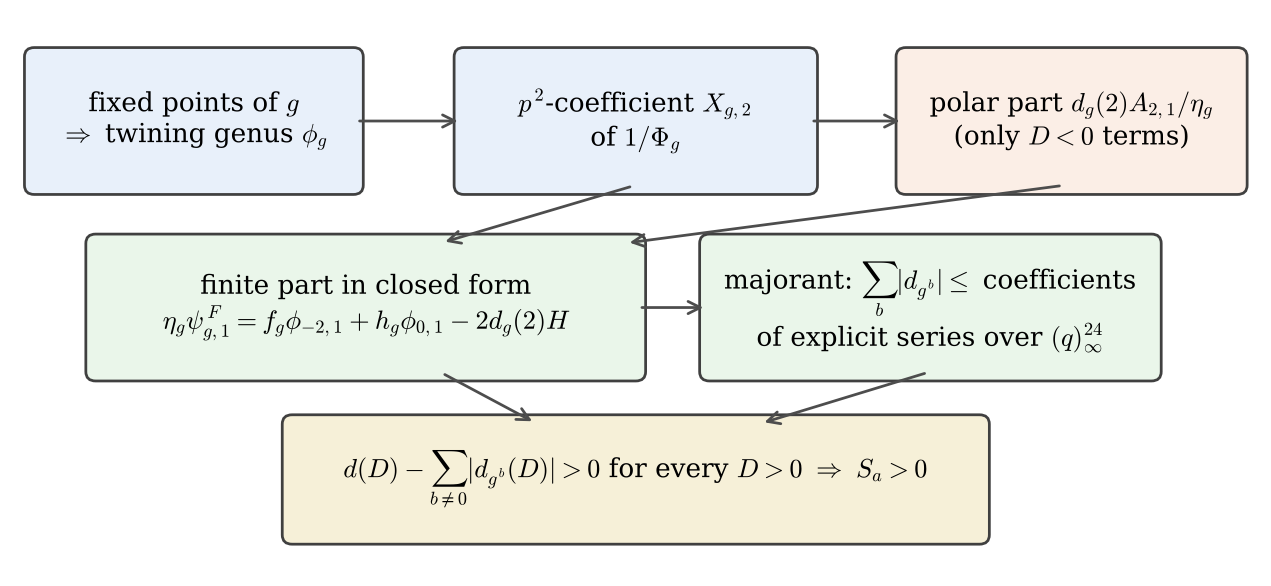
\includegraphics[width=0.93\textwidth]{figures/fig_flow.png}
\caption{Structure of the proof. The polar part of the Fourier--Jacobi coefficient is an Appell--Lerch sum which does not contribute in the attractor region; the finite part has the closed form of Theorem~\ref{thm:B}, and a coefficientwise majorant gives Theorem~\ref{thm:C}.}
\label{fig:flow}
\end{figure}

\subsection*{Notation}
Throughout, $\tau\in\HH$, $z\in\CC$, $q=e^{2\pi i\tau}$, $y=e^{2\pi iz}$ and $(q;q)_\infty=\prod_{n\ge1}(1-q^n)$; we write $(q)_\infty$ for short. For a power series $F(q)=\sum a_mq^m$ we write $[q^m]F=a_m$, and $|F|=\sum|a_m|q^m$. For two series with real coefficients, $F\preceq G$ means $[q^m]F\le[q^m]G$ for all $m$. If $0\preceq F\preceq G$ and $0\preceq F'\preceq G'$ then $FF'\preceq GG'$. We write $\sigma_k(m)=\sum_{d\mid m}d^k$, $\sigma=\sigma_1$, and $p_k(m)=[q^m](q)_\infty^{-k}$ for the number of $k$-coloured partitions. The Eisenstein series are $E_2=1-24\sum\sigma(m)q^m$, $E_4=1+240\sum\sigma_3(m)q^m$, and for $d\ge2$ we put
\[
\phi^{(d)}(\tau)=\frac{d\,E_2(d\tau)-E_2(\tau)}{d-1}\in M_2(\Gamma_0(d)).
\]

\section{Symplectic automorphisms and the twined partition function}\label{sec:setup}

\subsection{The seven types}
Let $X$ be a complex $K3$ surface and $g$ an automorphism of finite order $N>1$ preserving the holomorphic two-form. Nikulin proved that $g$ has finitely many fixed points, that $N\le 8$, and that the number of fixed points depends only on $N$: it is $8,6,4,4,2,3,2$ for $N=2,\dots,8$ \cite{Nik79}. At a fixed point $g$ acts on the tangent space by $\operatorname{diag}(\zeta,\zeta^{-1})$ with $\zeta$ a primitive root of unity of order dividing $N$, and the trace of $g$ on $H^*(X,\QQ)$ equals the number of fixed points. Mukai showed that the action of $g$ on $H^*(X,\QQ)\cong\QQ^{24}$ is that of an element of $M_{23}\subset M_{24}$ with at least five orbits on the $24$ points \cite{Muk88}; with Nikulin's fixed-point count this determines the cycle shape, and hence the conjugacy class in $M_{24}$, from $N$. The seven types are listed in Table~\ref{tab:classes}. Symplectic involutions and the Kummer and Enriques surfaces attached to them are discussed in \cite{BN26}, and $K3$-fibred Calabi--Yau threefolds, on which such automorphisms can act fibrewise, in \cite{Bha22}.

\begin{table}[H]
\centering
\caption{Symplectic automorphisms of $K3$. The cycle shape $\prod a^{m_a}$ is that of the permutation action on $\QQ^{24}$; the eta product is $\eta_g(\tau)=\prod_a\eta(a\tau)^{m_a}$, and $\chi_g$ is the number of fixed points. The local rotation angles $\alpha$ (with $\zeta=e^{2\pi i\alpha}$) are listed with multiplicity. The last column is the class of $g^2$.}
\label{tab:classes}
\renewcommand{\arraystretch}{1.15}
\begin{tabular}{cccccc}
\toprule
type & $N$ & cycle shape & $\chi_g$ & rotation angles at the fixed points & $g^2$\\
\midrule
$2A$ & 2 & $1^82^8$ & 8 & $\tfrac12$ ($8$ times) & $1A$\\
$3A$ & 3 & $1^63^6$ & 6 & $\tfrac13$ ($6$ times) & $3A$\\
$4B$ & 4 & $1^42^24^4$ & 4 & $\tfrac14$ ($4$ times) & $2A$\\
$5A$ & 5 & $1^45^4$ & 4 & $\tfrac15,\tfrac15,\tfrac25,\tfrac25$ & $5A$\\
$6A$ & 6 & $1^22^23^26^2$ & 2 & $\tfrac16,\tfrac16$ & $3A$\\
$7A$ & 7 & $1^37^3$ & 3 & $\tfrac17,\tfrac27,\tfrac37$ & $7A$\\
$8A$ & 8 & $1^22\,4\,8^2$ & 2 & $\tfrac18,\tfrac38$ & $4B$\\
\bottomrule
\end{tabular}
\end{table}

In each case $\sum_a a\,m_a=24$, so $\eta_g(\tau)=q\,P_g(q)$ with $P_g(q)=\prod_a(q^a;q^a)_\infty^{m_a}$. We put
\[
d_g(k)=[q^k]\,\frac{1}{P_g(q)}.
\]
For $k=2$ these numbers are $324,52,27,16,14,7,9,6$ for the classes $1A,2A,\dots,8A$. The total number of cycles $\sum_a m_a$ is at most $16$, and this will matter in Section~\ref{sec:majorant}. Since the type of $g^b$ depends only on $N/\gcd(b,N)$, the powers of $g$ are determined by the last column of Table~\ref{tab:classes} and by $g^3$ of type $2A$ for $g$ of type $6A$.

\subsection{Twining genera}
The twining genus $\phi_g(\tau,z)$ of $X$ is the trace of $g$ on the Ramond sector of the $K3$ sigma model weighted as in the elliptic genus; equivalently it is the $g$-equivariant elliptic genus of $X$. For $g=1$ it is $2\phi_{0,1}$. For every $g$ in Table~\ref{tab:classes}, $\phi_g$ is a weak Jacobi form of weight $0$ and index $1$ for $\Gamma_0(N)$ with trivial character \cite{Che10,GHV10}.

\begin{proposition}\label{prop:genus}
With $\chi_g$ and $T_g\in M_2(\Gamma_0(N))$ as in Table~\ref{tab:Tg},
\[
\phi_g=\frac{\chi_g}{12}\,\phi_{0,1}+T_g\,\phi_{-2,1}.
\]
\end{proposition}

The proof is in Appendix~\ref{app:genus}. The formula agrees with the twining genera of Mathieu moonshine. With $\Lambda_d=\frac{d}{24}\bigl(dE_2(d\tau)-E_2(\tau)\bigr)=\frac{d(d-1)}{24}\phi^{(d)}$, the forms of Table~\ref{tab:Tg} are $16\Lambda_2$, $6\Lambda_3$, $4(\Lambda_4-\Lambda_2)$, $2\Lambda_5$, $2(\Lambda_6-\Lambda_3-\Lambda_2)$, $\Lambda_7$ and $\Lambda_8-\Lambda_4$, which is the form in which the weight-two parts of the twining genera appear in \cite{Che10,GHV10}.\footnote{Our proof does not use moonshine: Proposition~\ref{prop:genus} is derived from the fixed points alone, and the comparison with \cite{Che10,GHV10} is only a consistency check.}

\begin{table}[H]
\centering
\caption{The weight-two forms $T_g$ of Proposition~\ref{prop:genus}.}
\label{tab:Tg}
\renewcommand{\arraystretch}{1.2}
\begin{tabular}{cccccccc}
\toprule
$g$ & $2A$ & $3A$ & $4B$ & $5A$ & $6A$ & $7A$ & $8A$\\
\midrule
$T_g$ & $\tfrac43\phi^{(2)}$ & $\tfrac32\phi^{(3)}$ & $-\tfrac13\phi^{(2)}+2\phi^{(4)}$ & $\tfrac53\phi^{(5)}$ & $-\tfrac16\phi^{(2)}-\tfrac12\phi^{(3)}+\tfrac52\phi^{(6)}$ & $\tfrac74\phi^{(7)}$ & $-\tfrac12\phi^{(4)}+\tfrac73\phi^{(8)}$\\
\bottomrule
\end{tabular}
\end{table}

\subsection{The twined partition function}
Write $\phi_g=\sum c_g(n,\ell)q^ny^\ell$ and put $p=e^{2\pi i\sigma}$ for a third variable $\sigma\in\HH$. The generating function of the twined indices of quarter-BPS dyons is $1/\Phi_g(\tau,z,\sigma)$, where \cite{DJS07,Sen10,Che10,PV14}
\begin{equation}\label{eq:Phig}
\frac{1}{\Phi_g}=\frac{1}{p\,\eta_g(\tau)\,\phi_{-2,1}(\tau,z)}\exp\Bigl(\sum_{k\ge1}\sum_{r\ge1}\sum_{n\ge0}\sum_{\ell\in\ZZ}\frac1k\,c_{g^k}(rn,\ell)\,\bigl(p^rq^ny^\ell\bigr)^k\Bigr).
\end{equation}
This is the second-quantised twining genus of Dijkgraaf, Moore, Verlinde and Verlinde \cite{DMVV97} multiplied by the contribution of the centre of mass and of the Kaluza--Klein monopole. Raum and Persson--Volpato proved that $\Phi_g$ is a Siegel modular form for a level-$N$ subgroup of $\mathrm{Sp}_4(\ZZ)$ \cite{Rau13,PV14}; we do not use modularity in the variable $\sigma$.

Expanding \eqref{eq:Phig} in powers of $p$ gives $1/\Phi_g=\sum_{m\ge-1}\psi_{g,m}\,p^m$ with $\psi_{g,m}=X_{g,m+1}/(\eta_g\phi_{-2,1})$, where $X_{g,0}=1$, $X_{g,1}=\phi_g$ and
\begin{equation}\label{eq:X2}
X_{g,2}(\tau,z)=\tfrac12\,\phi_g(\tau,z)^2+\bigl(U_2\phi_g\bigr)(\tau,z)+\tfrac12\,\phi_{g^2}(2\tau,2z),\qquad U_2\phi=\sum_{n,\ell}c(2n,\ell)\,q^ny^\ell .
\end{equation}
The three terms come from $(k,r)=(1,1)$ squared, $(k,r)=(1,2)$, and $(k,r)=(2,1)$. The function $\psi_{g,m}$ is the generating function of twined indices of magnetic charge $P^2/2=m$. In this paper $m=1$, and we abbreviate $\psi_g=\psi_{g,1}$.

\subsection{The attractor contour}
The index of a dyon with charges $(n,\ell,m)$ is a Fourier coefficient of $1/\Phi_g$, but the coefficient depends on the region in which the meromorphic function is expanded, because of wall crossing. Sen's attractor contour selects the expansion adapted to the attractor values of the moduli, and the resulting coefficients are the indices of single-centred black holes \cite{Sen07,CV08,BSS09}. For the Fourier--Jacobi coefficient $\psi_{g,m}$ this means: expand $\psi_{g,m}$ in powers of $q$ and $y$ in the strip of $z$ containing the point $z=-\ell\tau/(2m)$ and take the coefficient of $q^ny^\ell$.\footnote{The attractor value of $\operatorname{Im}z/\operatorname{Im}\tau$ is $-\ell/(2m)$; see \cite[Section~8]{Sen07} and \cite[Section~2]{BSS09}. In \cite{GSSV23} the same prescription appears as the condition $0\le Q\cdot P\le\min(Q^2,P^2)$ together with an expansion in $e^{-2\pi iv}$; for $m=1$ this is the strip $-\operatorname{Im}\tau<\operatorname{Im}z<0$, and Lemma~\ref{lem:strip} below shows that it gives the same numbers.} When $\ell/(2m)$ is an integer the point lies on a line of poles and either adjacent strip may be used; Lemma~\ref{lem:strip} shows that the answer is the same.

\begin{definition}\label{def:index}
Let $D=4n-\ell^2>0$. The \emph{twined single-centred index} of a $g$-invariant dyon with $Q^2/2=n$, $Q\cdot P=\ell$ and $P^2/2=1$ is
\[
d_g(n,\ell)=(-1)^{\ell+1}\,\bigl[q^ny^\ell\bigr]\,\psi_g\big|_{S},
\]
where $\psi_g|_S$ denotes the Fourier expansion of $\psi_g$ in a strip $S=\{-(s+1)\operatorname{Im}\tau<\operatorname{Im}z<-s\operatorname{Im}\tau\}$, $s\in\ZZ$, whose closure contains $-\ell\tau/2$. We write $d=d_1$.
\end{definition}

The sign $(-1)^{\ell+1}$ removes the contribution of the fermion zero modes; with it $d_g=-B_6^{g}$ in the notation of \cite{GSSV23}. The discrete information is $S_a=\frac1N\sum_be^{-2\pi iab/N}d_{g^b}(n,\ell)$.

\section{The twined single-centred index}\label{sec:finite}

\subsection{The polar part}
Let
\[
A_{2,1}(\tau,z)=\sum_{s\in\ZZ}\frac{q^{s^2+s}y^{2s+1}}{(1-q^sy)^2}.
\]
This is the Appell--Lerch sum of \cite[Section~3]{BM13} for $m=1$. It is meromorphic in $z$ with double poles exactly at $z\in\ZZ+\tau\ZZ$, and near $z=0$ the term $s=0$ gives $A_{2,1}=y/(1-y)^2+O(1)=1/(2\pi iz)^2+O(1)$.\footnote{The other terms are holomorphic at $z=0$ since $q^s\ne1$ for $s\ne0$. The leading behaviour of $y/(1-y)^2$ at $y=1$ is $1/(2\pi iz)^2$, and $y/(1-y)^2$ is even in $z$, so there is no simple pole.}

\begin{lemma}\label{lem:strip}
Let $s_0\in\ZZ$ and expand $A_{2,1}$ in the strip $S_{s_0}=\{-(s_0+1)\operatorname{Im}\tau<\operatorname{Im}z<-s_0\operatorname{Im}\tau\}$. Every monomial $q^ny^\ell$ that occurs has $4n-\ell^2=-(k+1)^2$ for some integer $k\ge0$, and no monomial with $\ell\in\{2s_0,2s_0+1,2s_0+2\}$ occurs.
\end{lemma}

\begin{proof}
In $S_{s_0}$ one has $|q^sy|<1$ if and only if $s\operatorname{Im}\tau+\operatorname{Im}z>0$, that is, if and only if $s\ge s_0+1$. For such $s$,
\[
\frac{q^{s^2+s}y^{2s+1}}{(1-q^sy)^2}=\sum_{k\ge0}(k+1)\,q^{s^2+s+ks}\,y^{2s+1+k},
\]
and the exponents satisfy $4(s^2+s+ks)-(2s+1+k)^2=-(k+1)^2$ and $\ell=2s+1+k\ge2s_0+3$. For $s\le s_0$ one has $|q^sy|>1$, and
\[
\frac{q^{s^2+s}y^{2s+1}}{(1-q^sy)^2}=\sum_{k\ge0}(k+1)\,q^{s^2+s-s(k+2)}\,y^{2s+1-(k+2)},
\]
with $4(s^2-s(k+1))-(2s-k-1)^2=-(k+1)^2$ and $\ell=2s-k-1\le2s_0-1$. Hence every exponent $\ell$ lies outside $\{2s_0,2s_0+1,2s_0+2\}$.
\end{proof}

If $\ell$ is odd, the attractor point $-\ell\tau/2$ lies in the strip $S_{(\ell-1)/2}$, and $\ell=2s_0+1$. If $\ell$ is even, it lies on the boundary of $S_{\ell/2}$ and $S_{\ell/2-1}$, and $\ell$ equals $2s_0$ in the first and $2s_0+2$ in the second. In all cases $\ell$ is one of the three excluded exponents of the strip used in Definition~\ref{def:index}.

\subsection{The finite part}
Let $\phi_{-2,1}=A$ and $\phi_{0,1}=B$ be the weak Jacobi forms
\[
A=(y-2+y^{-1})\prod_{n\ge1}\frac{(1-q^ny)^2(1-q^ny^{-1})^2}{(1-q^n)^4},\qquad
B=4\sum_{i=2}^4\frac{\vt_i(\tau,z)^2}{\vt_i(\tau,0)^2},
\]
so that $A=(2\pi iz)^2+O(z^4)$ and $B(\tau,0)=12$ \cite[Section~9]{EZ85}. Let
\[
\cH(\tau,z)=\sum_{n\ge0}\sum_{\ell\in\ZZ}H(4n-\ell^2)\,q^ny^\ell,
\]
where $H(0)=-\tfrac1{12}$, $H(N)$ for $N>0$ is the Hurwitz class number (the number of $\mathrm{SL}_2(\ZZ)$-classes of positive definite binary quadratic forms of discriminant $-N$, those equivalent to multiples of $x^2+y^2$ or $x^2+xy+y^2$ counted with weight $\frac12$ or $\frac13$), and $H(N)=0$ if $N<0$ or $N\equiv1,2\pmod4$ \cite{HZ76,Zag08}.

\begin{proposition}[Dabholkar--Murthy--Zagier]\label{prop:DMZ}
As meromorphic functions,
\[
\frac{B^2-E_4A^2}{144\,A}=A_{2,1}-2\,\cH .
\]
\end{proposition}

This identity is the case $m=1$ of the decomposition of $B^{m+1}/A$ into polar and finite parts; it is stated as $(B^2/A)^F=E_4A-288\,\cH$ in \cite[Section~3]{BM13}, where $(B^2/A)^F=B^2/A-144\,A_{2,1}$.\footnote{The polar part of $B^2/A$ is $144\,A_{2,1}$ because $B(\tau,0)^2=144$. Both sides of Proposition~\ref{prop:DMZ} have the same double poles; their difference is holomorphic in $z$ and transforms as a Jacobi form of weight two and index one up to the shadow of $\cH$, which is Zagier's weight-$\frac32$ Eisenstein series \cite{HZ76}. We have also checked the identity coefficient by coefficient for all exponents of $q$ up to $99$, expanding $A_{2,1}$ in the strip $-\operatorname{Im}\tau<\operatorname{Im}z<0$; the program is in the archive \cite{Bha26}.} We now derive the twined analogue.

\begin{proposition}\label{prop:W}
Put $W_g=\bigl(X_{g,2}-\tfrac{d_g(2)}{144}(B^2-E_4A^2)\bigr)/A$. Then $W_g$ is holomorphic on $\HH\times\CC$, and
\begin{equation}\label{eq:split}
\eta_g\,\psi_g=W_g-2\,d_g(2)\,\cH+d_g(2)\,A_{2,1}.
\end{equation}
\end{proposition}

\begin{proof}
The identity \eqref{eq:split} is the definition of $W_g$ combined with Proposition~\ref{prop:DMZ}, since $\eta_g\psi_g=X_{g,2}/A$. For holomorphy, $A$ vanishes exactly on $\ZZ+\tau\ZZ$, to order two \cite[Theorem~9.3]{EZ85}, and the numerator $N_g=X_{g,2}-\frac{d_g(2)}{144}(B^2-E_4A^2)$ satisfies the elliptic transformation law of index two, $N_g(\tau,z+\lambda\tau+\mu)=q^{-2\lambda^2}y^{-4\lambda}N_g(\tau,z)$; so the order of vanishing of $N_g$ is the same at all points of $\ZZ+\tau\ZZ$, and it suffices to show that $N_g$ vanishes to order two at $z=0$. All functions involved are even in $z$, so $N_g$ has no linear term. At $z=0$ we have $\phi_g(\tau,0)=\chi_g$ and $\phi_{g^2}(\tau,0)=\chi_{g^2}$ (the Euler characteristic of the fixed locus), and $(U_2\phi_g)(\tau,0)=\sum_n\bigl(\sum_\ell c_g(2n,\ell)\bigr)q^n=\chi_g$. Hence
\[
X_{g,2}(\tau,0)=\tfrac12\chi_g^2+\chi_g+\tfrac12\chi_{g^2}.
\]
On the other hand, at $z=0$ only the terms with $n=0$ survive in \eqref{eq:Phig}, because $\sum_\ell c_{g^k}(j,\ell)=\chi_{g^k}\delta_{j,0}$, so $X_{g,2}(\tau,0)$ is the coefficient of $p^2$ in
\[
\exp\Bigl(\sum_{r\ge1}\sum_{k\ge1}\frac1k\,\chi_{g^k}\,p^{rk}\Bigr)=\prod_{r\ge1}\prod_a\bigl(1-p^{ar}\bigr)^{-m_a}=\frac{1}{P_g(p)}.
\]
The middle identity follows from $\chi_{g^k}=\sum_{a\mid k}a\,m_a$, the number of points of $\{1,\dots,24\}$ fixed by $g^k$, which gives $\sum_k\frac1k\chi_{g^k}x^k=-\sum_am_a\log(1-x^a)$. Therefore $X_{g,2}(\tau,0)=[p^2]\,P_g(p)^{-1}=d_g(2)$, which equals $\frac{d_g(2)}{144}B(\tau,0)^2$. So $N_g(\tau,0)=0$.
\end{proof}

\begin{theorem}\label{thm:finite}
Let $\psi^F_g=(W_g-2\,d_g(2)\,\cH)/\eta_g=\sum c^F_g(n,\ell)q^ny^\ell$. Then $c^F_g(n,\ell)=C^F_g(4n-\ell^2)$ depends only on the discriminant, and for every $(n,\ell)$ with $D=4n-\ell^2>0$,
\[
d_g(n,\ell)=(-1)^{\ell+1}\,C^F_g(D)=(-1)^{D+1}\,C^F_g(D).
\]
\end{theorem}

\begin{proof}
By Proposition~\ref{prop:W}, $\psi_g=\psi^F_g+d_g(2)A_{2,1}/\eta_g$. The function $\psi^F_g$ is holomorphic in $z$, so its Fourier expansion is the same in every strip. The second term is $d_g(2)\,q^{-1}P_g(q)^{-1}A_{2,1}$, and multiplication by a power series in $q$ does not change the exponent of $y$. By Lemma~\ref{lem:strip} the expansion of $A_{2,1}$ in the strip of Definition~\ref{def:index} contains no monomial with exponent $\ell$ of $y$, so the coefficient of $q^ny^\ell$ of $\psi_g|_S$ equals $c^F_g(n,\ell)$. That $c^F_g$ depends only on $4n-\ell^2$ follows from the elliptic invariance of $W_g$ (Proposition~\ref{prop:W}) and of $\cH$; it is shown concretely by the theta decomposition in Section~\ref{sec:closed}. Finally $D\equiv-\ell^2\equiv\ell\pmod2$.
\end{proof}

Theorem~\ref{thm:finite} shows in particular that the twined indices of magnetic charge one do not depend on the choice of strip, a fact also visible in the tables of \cite{GSSV23}. For $g=1$ it recovers $d(n,\ell)=(-1)^{\ell+1}C^F_1(D)$ with $\Delta\psi^F_1=3E_4A-648\,\cH$ \cite{BM13}.

\section{The closed form}\label{sec:closed}

\subsection{Weak Jacobi forms of index one}
Let $\Gamma\subset\mathrm{SL}_2(\ZZ)$ be a congruence subgroup. A weak Jacobi form of weight $k$ and index one for $\Gamma$ is a holomorphic function on $\HH\times\CC$ with the usual transformation laws under $\Gamma$ and under $z\mapsto z+\lambda\tau+\mu$, whose Fourier expansion at every cusp contains only non-negative powers of $q$.

\begin{lemma}\label{lem:structure}
Let $k$ be even and $W$ a weak Jacobi form of weight $k$ and index one for $\Gamma$, even in $z$. Then $W=f\,A+h\,B$ with $h=W(\tau,0)/12\in M_k(\Gamma)$ and $f\in M_{k+2}(\Gamma)$. If $W=\sum_n\sum_\ell w(n,\ell)q^ny^\ell$ and $\mu_j(W)=\sum_n\bigl(\sum_\ell w(n,\ell)\ell^{2j}\bigr)q^n$, then
\begin{equation}\label{eq:moments}
h=\tfrac1{12}\,\mu_0(W),\qquad f=\tfrac12\bigl(\mu_1(W)-2E_2\,h\bigr).
\end{equation}
\end{lemma}

\begin{proof}
The function $h(\tau)=W(\tau,0)/12$ is a modular form of weight $k$ for $\Gamma$, holomorphic at the cusps since $W$ is weak. The function $W-hB$ is a weak Jacobi form of weight $k$ and index one, even in $z$, vanishing at $z=0$, hence vanishing to order two at every point of $\ZZ+\tau\ZZ$. Since $A$ has exactly these zeros, each of order two, $f=(W-hB)/A$ is holomorphic, transforms like a Jacobi form of weight $k+2$ and index zero, and is therefore independent of $z$: a holomorphic function that is invariant under $z\mapsto z+\lambda\tau+\mu$ is bounded in $z$. So $f\in M_{k+2}(\Gamma)$; the behaviour at the cusps is controlled by \eqref{eq:moments}, which expresses $f$ through coefficients of $W$ at each cusp. For \eqref{eq:moments}, write $W=\sum_j\frac{(2\pi iz)^{2j}}{(2j)!}\mu_j(W)$, and use $A=(2\pi iz)^2+O(z^4)$, $B=12+\mu_1(B)\frac{(2\pi iz)^2}{2}+O(z^4)$ with $\mu_1(B)=2E_2$.\footnote{From $B=12+(2\pi iz)^2E_2+O(z^4)$; see \cite[Section~9]{EZ85}. The coefficient of $(2\pi iz)^2/2$ in $fA+hB$ is $2f+2E_2h$.} Comparing the coefficients of $(2\pi iz)^0$ and $(2\pi iz)^2/2$ gives $\mu_0(W)=12h$ and $\mu_1(W)=2f+2E_2h$.
\end{proof}

\begin{proposition}\label{prop:Wweak}
$W_g$ is a weak Jacobi form of weight $2$ and index one for $\Gamma(4N)$, even in $z$.
\end{proposition}

\begin{proof}
Each of $\phi_g(\tau,z)^2$, $\phi_g(\tau/2,z)$, $\phi_g((\tau+1)/2,z)$ and $\phi_{g^2}(2\tau,2z)$ is a weak Jacobi form of weight $0$ and index $2$ for $\Gamma(4N)$. For the middle two, $\gamma=\left(\begin{smallmatrix}a&b\\c&d\end{smallmatrix}\right)\in\Gamma(4N)$ acts on $\tau/2$ through $\left(\begin{smallmatrix}a&b/2\\2c&d\end{smallmatrix}\right)\in\Gamma_0(N)$, and on $(\tau+1)/2$ through $\left(\begin{smallmatrix}a+c&(b+d-a-c)/2\\2c&d-c\end{smallmatrix}\right)\in\Gamma_0(N)$; for the last, through $\left(\begin{smallmatrix}a&2b\\c/2&d\end{smallmatrix}\right)\in\Gamma_0(N)$. At any cusp, $\gamma'\in\mathrm{SL}_2(\ZZ)$ composed with $\tau\mapsto\tau/2$ factors as an element of $\mathrm{SL}_2(\ZZ)$ followed by an upper triangular rational map, so the expansion at the cusp has only non-negative powers of $q$ because $\phi_g$ is weak at all cusps \cite{Che10,GHV10}. Hence $X_{g,2}=\frac12\phi_g^2+\frac12\bigl(\phi_g(\frac\tau2,z)+\phi_g(\frac{\tau+1}2,z)\bigr)+\frac12\phi_{g^2}(2\tau,2z)$ is weak of index two for $\Gamma(4N)$. Since $B^2-E_4A^2$ is a weak Jacobi form of weight $0$ and index $2$ for $\mathrm{SL}_2(\ZZ)$ and $A$ one of weight $-2$ and index one, $W_g$ transforms with weight $2$ and index one and is holomorphic by Proposition~\ref{prop:W}. Its behaviour at the cusps follows from the moment formulas of Lemma~\ref{lem:structure} applied to $N_g=AW_g$: the Taylor coefficients of $W_g$ in $z$ are finite combinations of the moments of $N_g$ and of the quasimodular series $E_2$, which have only non-negative powers of $q$ at every cusp.
\end{proof}

\begin{proof}[Proof of Theorem~\ref{thm:B}]
By Lemma~\ref{lem:structure} and Proposition~\ref{prop:Wweak}, $W_g=f\,A+h\,B$ with $f\in M_4(\Gamma(4N))$ and $h\in M_2(\Gamma(4N))$, and \eqref{eq:moments} computes the $q$-expansions of $f$ and $h$ from that of $X_{g,2}$, which in turn is given by Proposition~\ref{prop:genus} and \eqref{eq:X2}. Both $f$ and $h$ have integral exponents of $q$, because $U_2$ and $\tau\mapsto2\tau$ preserve integrality of exponents. Let $f_g,h_g$ be the forms of Table~\ref{tab:fh}; they lie in $M_4(\Gamma_0(N))$ and $M_2(\Gamma_0(N))$. By Sturm's theorem \cite{Stu87}, a modular form of weight $k$ for $\Gamma(M)$, $M\ge3$, whose expansion in $q$ vanishes to order greater than $\frac{k}{24}M^2\prod_{p\mid M}(1-p^{-2})$ is zero.\footnote{Sturm's bound is $\frac{k}{12}[\mathrm{SL}_2(\ZZ):\Gamma(M)]/2$ in the local parameter $q^{1/M}$ at $\infty$, and $[\mathrm{PSL}_2(\ZZ):\overline{\Gamma(M)}]=\frac{M^3}{2}\prod_{p\mid M}(1-p^{-2})$ for $M\ge3$. Dividing by $M$ converts to powers of $q$.} For $M=4N\le 32$ and $k=4$ this order is at most $128$. The $q$-expansions of $f-f_g$ and $h-h_g$ vanish beyond this order (the bound plus one for each type, which is $q^{129}$ for $8A$) by exact rational arithmetic (Appendix~\ref{app:code}). Hence $f=f_g$ and $h=h_g$. Theorem~\ref{thm:finite} completes the proof.
\end{proof}

\begin{table}[H]
\centering
\caption{The forms $f_g\in M_4(\Gamma_0(N))$ and $h_g\in M_2(\Gamma_0(N))$ of Theorem~\ref{thm:B}, with $E_4^{(d)}(\tau)=E_4(d\tau)$.}
\label{tab:fh}
\renewcommand{\arraystretch}{1.3}
\begin{tabular}{cll}
\toprule
$g$ & $f_g$ & $h_g$\\
\midrule
$1A$ & $3E_4$ & $0$\\
$2A$ & $\tfrac7{15}E_4+\tfrac{64}{45}E_4^{(2)}$ & $\tfrac{10}9\phi^{(2)}$\\
$3A$ & $\tfrac{57}{160}E_4+\tfrac{243}{160}E_4^{(3)}$ & $\tfrac98\phi^{(3)}$\\
$4B$ & $\tfrac7{30}E_4-\tfrac{14}{45}E_4^{(2)}+\tfrac{32}{15}E_4^{(4)}$ & $-\tfrac1{18}\phi^{(2)}+\phi^{(4)}$\\
$5A$ & $\tfrac1{32}E_4-\tfrac{625}{288}E_4^{(5)}+\tfrac{25}6\bigl(\phi^{(5)}\bigr)^2$ & $\tfrac{35}{36}\phi^{(5)}$\\
$6A$ & $\tfrac{33}{160}E_4-\tfrac{14}{45}E_4^{(2)}-\tfrac{117}{160}E_4^{(3)}+\tfrac{18}5E_4^{(6)}-\tfrac12\phi^{(2)}\phi^{(3)}$ & $-\tfrac1{18}\phi^{(2)}-\tfrac1{24}\phi^{(3)}+\tfrac56\phi^{(6)}$\\
$7A$ & $\tfrac{31}{960}E_4-\tfrac{2401}{960}E_4^{(7)}+\tfrac{147}{32}\bigl(\phi^{(7)}\bigr)^2$ & $\tfrac78\phi^{(7)}$\\
$8A$ & $\tfrac7{36}E_4^{(2)}-\tfrac8{15}E_4^{(4)}+\tfrac{64}{45}E_4^{(8)}+\tfrac76\phi^{(2)}\phi^{(8)}$ & $-\tfrac1{36}\phi^{(2)}+\tfrac79\phi^{(8)}$\\
\bottomrule
\end{tabular}
\end{table}

\subsection{Theta decomposition}
Let $\vt_{1,\mu}(\tau,z)=\sum_{r\equiv\mu\,(2)}q^{r^2/4}y^r$ and $\vt_\mu(\tau)=\vt_{1,\mu}(\tau,0)$ for $\mu\in\{0,1\}$, so that $\vt_0=\sum_{s\in\ZZ}q^{s^2}$ and $\vt_1=2q^{1/4}\Theta(q)$ with $\Theta(q)=\sum_{k\ge0}q^{k(k+1)}$. Every function $F=\sum c(n,\ell)q^ny^\ell$ with $c(n,\ell)=C(4n-\ell^2)$ can be written $F=F_0\vt_{1,0}+F_1\vt_{1,1}$ with $F_\mu(\tau)=\sum_{D\equiv-\mu^2\,(4)}C(D)q^{D/4}$. A direct computation, using $\eta(\tau)^6=q^{1/4}(q)_\infty^6$ and the heat equation for theta functions, gives \cite[Section~4]{BM13}
\begin{align*}
A&=\frac{-\vt_1\,\vt_{1,0}+\vt_0\,\vt_{1,1}}{\eta^6},&
B&=\frac{(24\vt_1'-E_2\vt_1)\,\vt_{1,0}+(E_2\vt_0-24\vt_0')\,\vt_{1,1}}{\eta^6},\\
\cH&=\cH_0\,\vt_{1,0}+\cH_1\,\vt_{1,1},&
\cH_0&=\sum_{n\ge0}H(4n)q^n,\quad \cH_1=q^{-1/4}\cH_1^\flat,\quad\cH_1^\flat=\sum_{n\ge1}H(4n-1)q^n,
\end{align*}
where $'=q\,\frac{d}{dq}$. Writing $\vt_1'=2q^{1/4}\Theta_1$ with $\Theta_1(q)=\sum_{k\ge0}\bigl(k^2+k+\tfrac14\bigr)q^{k(k+1)}$, and using $\eta_g=qP_g$, we obtain from Theorem~\ref{thm:B} the following explicit formulas. For $D=4n'$, $n'\ge1$,
\begin{equation}\label{eq:d0}
d_g(4n')=[q^{n'+1}]\,\Bigl(\frac{2f_g\Theta-2h_g\Theta_B}{(q)_\infty^6P_g}+\frac{2d_g(2)\,\cH_0}{P_g}\Bigr),\qquad\Theta_B=24\,\Theta_1-E_2\,\Theta,
\end{equation}
and for $D=4n'-1$, $n'\ge1$,
\begin{equation}\label{eq:d1}
d_g(4n'-1)=[q^{n'+1}]\,\Bigl(\frac{f_g\vt_0+h_g\,(E_2\vt_0-24\vt_0')}{(q)_\infty^6P_g}-\frac{2d_g(2)\,\cH_1^\flat}{P_g}\Bigr).
\end{equation}
Indeed, the $\vt_{1,0}$-component of $\eta_g\psi^F_g$ is $-2f_g\Theta/(q)_\infty^6+2h_g\Theta_B/(q)_\infty^6-2d_g(2)\cH_0$, the coefficient of $q^{n'}$ of $\psi^F_{g,0}$ is $C^F_g(4n')$, and $d_g(4n')=-C^F_g(4n')$ by Theorem~\ref{thm:finite}. The case $\mu=1$ is the same with $d_g=+C^F_g$ and an extra factor $q^{-1/4}$ absorbed by $\vt_0$ and $\cH_1^\flat$. For $g=1$, \eqref{eq:d0} and \eqref{eq:d1} become
\[
d(4n')=[q^{n'+1}]\Bigl(\frac{6E_4\Theta}{(q)^{30}_\infty}+\frac{648\,\cH_0}{(q)^{24}_\infty}\Bigr),\qquad
d(4n'-1)=[q^{n'+1}]\Bigl(\frac{3E_4\vt_0}{(q)^{30}_\infty}-\frac{648\,\cH_1^\flat}{(q)^{24}_\infty}\Bigr),
\]
the formulas of \cite[Section~4]{BM13}. Table~\ref{tab:values} lists the first values. For $2A$, $3A$ and $4B$ they agree with the values of $-B_6^{g}$ in Tables~3, 6 and~9 of \cite{GSSV23}.

\section{A majorant for the twined indices}\label{sec:majorant}

\subsection{The comparison series}
For $g$ of order $N\ge2$ put, with all absolute values taken coefficientwise,
\begin{align}
R_0&=\sum_{b=1}^{N-1}\bigl|2f_{g^b}\Theta-2h_{g^b}\Theta_B\bigr|,&
R_1&=\sum_{b=1}^{N-1}\bigl|f_{g^b}\vt_0+h_{g^b}(E_2\vt_0-24\vt_0')\bigr|,\label{eq:R}
\end{align}
and $H_\Sigma=\sum_{b=1}^{N-1}2\,d_{g^b}(2)$. Define
\begin{align}
k_0&=\frac{6E_4\Theta}{(q)_\infty^6}+648\,\cH_0-R_0-H_\Sigma\,|\cH_0|,\label{eq:k0}\\
k_1&=\frac{3E_4\vt_0}{(q)_\infty^6}-(648+H_\Sigma)\,\cH_1^\flat-R_1.\label{eq:k1}
\end{align}

\begin{proposition}\label{prop:majorant}
For $g$ of order $N\ge2$, $\mu\in\{0,1\}$ and $D=4n'-\mu>0$,
\[
d(D)-\sum_{b=1}^{N-1}\bigl|d_{g^b}(D)\bigr|\ \ge\ [q^{n'+1}]\,\frac{k_\mu(q)}{(q)_\infty^{24}}.
\]
\end{proposition}

\begin{proof}
Take $\mu=0$. For each $b$, write $F_b=2f_{g^b}\Theta-2h_{g^b}\Theta_B$. Since $1/(q^a;q^a)_\infty$ counts partitions into parts divisible by $a$, $0\preceq 1/(q^a;q^a)_\infty\preceq1/(q)_\infty$, and therefore $0\preceq1/P_{g^b}\preceq(q)_\infty^{-\sum_am_a}\preceq(q)_\infty^{-16}\preceq(q)_\infty^{-18}$, using that $(q)_\infty^{-2}$ has non-negative coefficients and constant term one. Consequently
\[
\Bigl|[q^k]\frac{F_b}{(q)_\infty^6P_{g^b}}\Bigr|\le[q^k]\frac{|F_b|}{(q)_\infty^6P_{g^b}}\le[q^k]\frac{|F_b|}{(q)_\infty^{24}},\qquad
\Bigl|[q^k]\frac{\cH_0}{P_{g^b}}\Bigr|\le[q^k]\frac{|\cH_0|}{(q)_\infty^{24}} .
\]
By \eqref{eq:d0}, $|d_{g^b}(4n')|\le[q^{n'+1}](|F_b|+2d_{g^b}(2)|\cH_0|)/(q)_\infty^{24}$, and summing over $b$ and subtracting from the formula for $d(4n')$ gives the claim. The case $\mu=1$ is identical, using \eqref{eq:d1} and $H(N)\ge0$ for $N\ge1$.
\end{proof}

\subsection{Coloured partitions}
The next lemma turns a coefficient inequality for $k_\mu$ into positivity of $k_\mu/(q)_\infty^{24}$.

\begin{lemma}\label{lem:partitions}
For $k\ge1$ and $n\ge1$, $n\,p_k(n)=k\sum_{m=1}^n\sigma(m)\,p_k(n-m)$.
\end{lemma}

\begin{proof}
Apply $q\frac{d}{dq}$ to $\log(q)_\infty^{-k}=k\sum_{m\ge1}\sigma(m)q^m/m$, which follows from $-\log(1-q^j)=\sum_{r\ge1}q^{jr}/r$. This gives $q\frac{d}{dq}(q)^{-k}_\infty=(q)_\infty^{-k}\cdot k\sum_m\sigma(m)q^m$; compare coefficients of $q^n$ \cite[Chapter~1]{And84}.
\end{proof}

\begin{lemma}\label{lem:positivity}
Let $k(q)=\sum_{m\ge0}a_mq^m$ with real coefficients and suppose that
\begin{equation}\label{eq:cond}
a_m>\frac{24\,|a_0|\,\sigma(m)}{\max(m,2)}\qquad\text{for all }m\ge1 .
\end{equation}
Then $[q^n]\,k(q)/(q)_\infty^{24}>0$ for every $n\ge2$.
\end{lemma}

\begin{proof}
Let $n\ge2$. For $1\le m\le n$ we have $\max(m,2)\le n$, so \eqref{eq:cond} gives $a_m>24|a_0|\sigma(m)/n$. By Lemma~\ref{lem:partitions} with $k=24$,
\[
\sum_{m=0}^na_mp_{24}(n-m)>a_0\,p_{24}(n)+\frac{24|a_0|}{n}\sum_{m=1}^n\sigma(m)p_{24}(n-m)=a_0\,p_{24}(n)+|a_0|\,p_{24}(n)\ge0 .
\]
The inequality is strict because $p_{24}(n-1)>0$ and $a_1>24|a_0|/n$.
\end{proof}

Proposition~\ref{prop:majorant} is applied with $n=n'+1\ge2$, which is exactly the range $D\ge3$ of Lemma~\ref{lem:positivity}.

\section{Proof of Theorem~\ref{thm:C}}\label{sec:proofC}

By Proposition~\ref{prop:majorant} and Lemma~\ref{lem:positivity}, Theorem~\ref{thm:C} follows once \eqref{eq:cond} is established for the fourteen series $k_\mu$, one for each type $g\ne1$ and each $\mu\in\{0,1\}$. Their constant terms $a_0$ are listed in Table~\ref{tab:consts}; for $2A$ and $\mu=1$ one has $a_0=0$, and \eqref{eq:cond} then says $a_m>0$.

\subsection{Coefficient bounds}
Let $c_A$ be the sum over $b=1,\dots,N-1$ of the absolute values of the coefficients of $f_{g^b}$ in the basis of Table~\ref{tab:fh}, and $c_B$ the same for $h_{g^b}$ (Table~\ref{tab:consts}).

\begin{lemma}\label{lem:coeffs}
For $i\ge1$:
\begin{enumerate}
\item $|[q^i]\phi^{(d)}|\le24\,\sigma(i)$ and $|[q^i]E_2|\le24\,\sigma(i)$;
\item if $F$ is $E_4(d\tau)$, a product $\phi^{(a)}\phi^{(b)}$, or a product $\phi^{(d)}E_2$, then $|[q^i]F|\le240\,\sigma_3(i)\le289\,i^3$;
\item $\sigma(i)\le i\,(1+\log i)$;
\item $H(N)\le 4i$ for $1\le N\le 4i$.
\end{enumerate}
All the series in (1) and (2) have constant term $1$.
\end{lemma}

\begin{proof}
(1) $[q^i]\phi^{(d)}=24\bigl(\sigma(i)-d\,\sigma(i/d)\bigr)/(d-1)$, with $\sigma(i/d)=0$ if $d\nmid i$. Since $d\,\sigma(i/d)=\sum_{e\mid i/d}de$ is a sum over a subset of the divisors of $i$, $0\le\sigma(i)-d\sigma(i/d)\le\sigma(i)$, and $d-1\ge1$.
(2) For $E_4(d\tau)$ the coefficient is $240\sigma_3(i/d)\le240\sigma_3(i)$. For a product $FG$ of two series with constant term $1$ and $|[q^j]F|,|[q^j]G|\le24\sigma(j)$,
\[
|[q^i](FG)|\le48\sigma(i)+576\sum_{j=1}^{i-1}\sigma(j)\sigma(i-j)=48\sigma(i)+48\bigl(5\sigma_3(i)+(1-6i)\sigma(i)\bigr)\le240\sigma_3(i),
\]
by Ramanujan's identity $\sum_{j=1}^{i-1}\sigma(j)\sigma(i-j)=\frac1{12}\bigl(5\sigma_3(i)+(1-6i)\sigma(i)\bigr)$, which is the identity $E_2^2=E_4+12E_2'$ read coefficientwise \cite{Zag08}, and $96\le288i$. Finally $\sigma_3(i)\le\zeta(3)i^3<1.2021\,i^3$.
(3) $\sigma(i)/i=\sum_{d\mid i}1/d\le\sum_{d=1}^i1/d\le1+\log i$.
(4) Each reduced form $ax^2+bxy+cy^2$ of discriminant $-N$ has $|b|\le a\le c$, hence $3a^2\le N$; for fixed $a$ there are at most $a+1$ values of $b$, and $c$ is then determined. So $H(N)\le\sum_{a\le\sqrt{N/3}}(a+1)\le\frac N6+\frac32\sqrt{N/3}$, which is at most $4i$ for $N\le4i$.
\end{proof}

\begin{proposition}\label{prop:large}
Let $\mu_0=2$, $\mu_1=1$. For $m\ge1$ the $m$-th coefficient $a_m$ of $k_\mu$ satisfies
\[
a_m\ \ge\ \frac{\mu_\mu\,m^5}{40}-(2\sqrt m+2)\Bigl(289(c_A+c_B)m^3+576\,c_B\bigl(m+\tfrac14\bigr)m(1+\log m)\Bigr)-4m\bigl(648\,[\mu=1]+H_\Sigma\bigr).
\]
\end{proposition}

\begin{proof}
\emph{Main term.} Since $\Theta\succeq1$ and $\vt_0\succeq1$ have non-negative coefficients, $[q^m]\,6E_4\Theta/(q)^6_\infty\ge6\,[q^m]E_4/(q)_\infty^6\ge6\bigl(p_6(m)+240\sigma_3(m)\bigr)$, keeping only the two extreme terms of the convolution. Since $1/(1-q)^6\preceq1/(q)_\infty^6$, $p_6(m)\ge\binom{m+5}5>m^5/120$. So the main term of $k_0$ exceeds $m^5/20$ and that of $k_1$ exceeds $m^5/40$.

\emph{Class number terms.} In $k_0$ the term $648\,\cH_0$ has non-negative coefficients for $m\ge1$ and is dropped; $H_\Sigma|\cH_0|$ contributes at most $H_\Sigma H(4m)\le4mH_\Sigma$. In $k_1$ the coefficient of $(648+H_\Sigma)\cH_1^\flat$ is $(648+H_\Sigma)H(4m-1)\le4m(648+H_\Sigma)$.

\emph{The series $R_\mu$.} Consider $\mu=0$ and one $b$. The series $2\Theta$ has non-negative coefficients summing to at most $2(\sqrt m+1)$ over exponents $\le m$, since $k(k+1)\le m$ forces $k\le\sqrt m$. By Lemma~\ref{lem:coeffs}(2), every coefficient of $f_{g^b}$ of index $i\le m$ is at most $289c_{A,b}m^3$ in absolute value (for $i=0$ it is at most $c_{A,b}$), so $|[q^m](2f_{g^b}\Theta)|\le(2\sqrt m+2)\,289\,c_{A,b}\,m^3$. Likewise $|[q^m](2h_{g^b}E_2\Theta)|\le(2\sqrt m+2)\,289\,c_{B,b}\,m^3$. Finally $48\,h_{g^b}\Theta_1$ has coefficient
\[
\Bigl|\sum_{k(k+1)\le m}48\bigl(k^2+k+\tfrac14\bigr)[q^{m-k(k+1)}]h_{g^b}\Bigr|\le(\sqrt m+1)\cdot48\bigl(m+\tfrac14\bigr)\cdot24\,c_{B,b}\,m(1+\log m),
\]
by Lemma~\ref{lem:coeffs}(1),(3), since $|[q^i]h_{g^b}|\le24c_{B,b}\sigma(i)\le24c_{B,b}m(1+\log m)$ for $1\le i\le m$ and $|[q^0]h_{g^b}|\le c_{B,b}$. Summing over $b$ gives the bound for $[q^m]R_0$. For $\mu=1$ the series $\vt_0$ has coefficients summing to $2\lfloor\sqrt m\rfloor+1\le2\sqrt m+2$ over exponents $\le m$, and $24\vt_0'$ has coefficient $24s^2\le24(m+\frac14)$ at $q^{s^2}$; the same estimates apply.
\end{proof}

\begin{corollary}\label{cor:large}
For every type and every $\mu$, condition \eqref{eq:cond} holds for all $m\ge11000$.
\end{corollary}

\begin{proof}
By Lemma~\ref{lem:coeffs}(3), $\sigma(m)/\max(m,2)\le1+\log m$, so by Proposition~\ref{prop:large} it suffices that
\[
\frac{\mu_\mu}{40}>\frac{\rho(m)}{m^5},
\]
where
\begin{align*}
\rho(m)={}&(2\sqrt m+2)\Bigl(289(c_A+c_B)m^3+576c_B\bigl(m+\tfrac14\bigr)m(1+\log m)\Bigr)\\
&+4m\bigl(648[\mu=1]+H_\Sigma\bigr)+24|a_0|(1+\log m).
\end{align*}
The right side is a sum of terms $m^{-\alpha}(1+\log m)^\beta$, $m^{-\alpha}$ and $m^{-\alpha}(1+\frac1{4m})(1+\log m)$ with positive coefficients, $\alpha\ge3/2$ and $\beta\le1$; each is decreasing for $m\ge1$, because $\frac{d}{dm}\log\bigl(m^{-\alpha}(1+\log m)\bigr)=\frac1m\bigl(-\alpha+\frac1{1+\log m}\bigr)<0$. So the right side is decreasing, and it suffices to check the inequality at a single $m_0$. With the constants of Table~\ref{tab:consts} it holds at the values $m_0$ listed there, the largest being $m_0=10792$ for $7A$ and $\mu=1$; hence it holds for all $m\ge11000$.\footnote{At $m=m_0$ the ratio of the two sides is between $1.000005$ (for $5A$, $\mu=1$) and $1.0006$; it was evaluated with forty significant digits. The thresholds are not optimised.}
\end{proof}

\subsection{The remaining coefficients}
For $1\le m<11000$ the coefficients $a_m$ of the fourteen series $k_\mu$ are rational numbers that can be computed exactly from \eqref{eq:R}--\eqref{eq:k1}, Table~\ref{tab:fh} and the class numbers. We have computed all of them for $m\le12045$ in exact rational arithmetic and checked \eqref{eq:cond} for each (Appendix~\ref{app:code}). The smallest value of the ratio $a_m\max(m,2)/(24|a_0|\sigma(m))$ occurs at $m=1$ in every case and equals $1.333\ldots$ for $6A$ with $\mu=0$; the ratio grows faster than any power of $m$ (Figure~\ref{fig:margins}).

\begin{proof}[Proof of Theorem~\ref{thm:C}]
Let $D>0$ and write $D=4n'-\mu$ with $\mu\in\{0,1\}$ and $n'\ge1$ (the cases $D\equiv1,2\pmod 4$ do not occur). By Corollary~\ref{cor:large} and the exact computation, $k_\mu$ satisfies \eqref{eq:cond}. Lemma~\ref{lem:positivity} with $n=n'+1\ge2$ gives $[q^{n'+1}]k_\mu/(q)_\infty^{24}>0$, and Proposition~\ref{prop:majorant} gives $d(D)>\sum_{b\ne0}|d_{g^b}(D)|$.
\end{proof}

\begin{proof}[Proof of Theorem~\ref{thm:A}]
By Theorem~\ref{thm:finite}, $d_{g^b}(n,\ell)=d_{g^b}(D)$ depends only on $D$. By \eqref{eq:Sa} and Theorem~\ref{thm:C},
\[
N\,S_a=d(D)+\sum_{b=1}^{N-1}e^{-2\pi iab/N}d_{g^b}(D)\ge d(D)-\sum_{b=1}^{N-1}|d_{g^b}(D)|>0. \qedhere
\]
\end{proof}

\begin{remark}
The argument proves more than positivity of $S_a$: every linear combination $\sum_b\lambda_bd_{g^b}$ with $|\lambda_b|\le\lambda_0$ for $b\ne0$ and $\lambda_0>0$ is positive. In particular the indices twined by characters of the cyclic group $\langle g\rangle$ and by sums of such characters are positive. The integrality of $S_a$ is not used. We have checked that $S_a$ is an integer for all $D\le600$ and every type; we do not prove integrality in general.
\end{remark}

\begin{figure}[t]
\centering
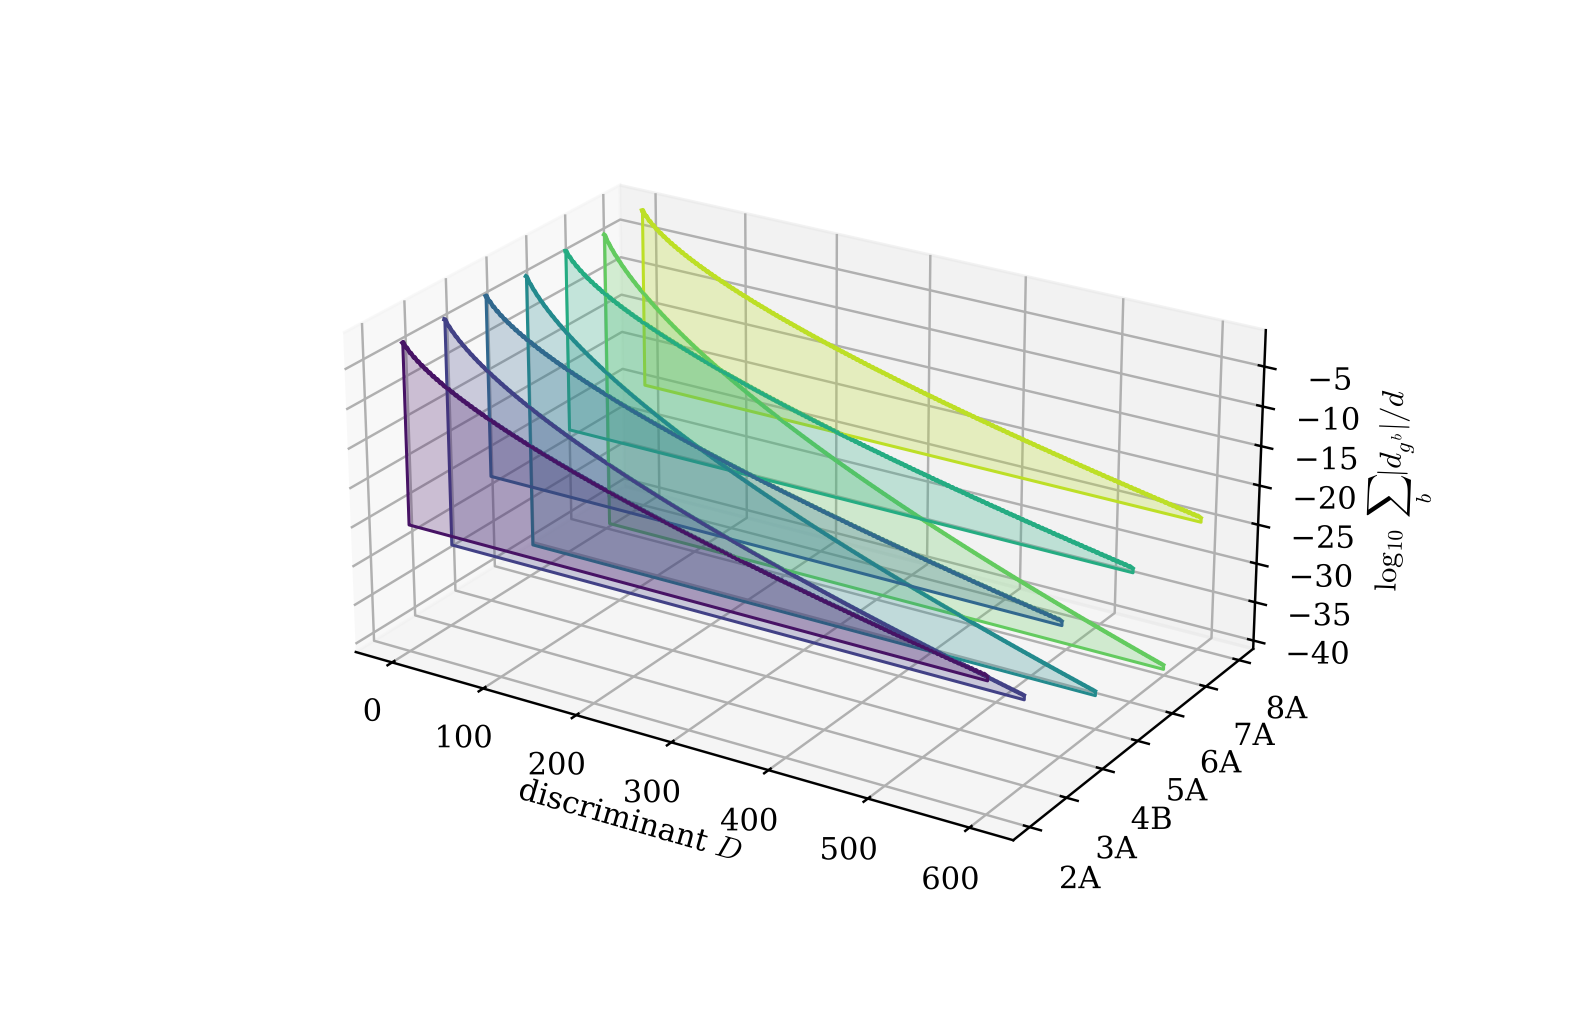
\includegraphics[width=0.9\textwidth]{figures/fig_ratio.png}
\caption{The ratio $\sum_{b\ne0}|d_{g^b}(D)|/d(D)$ for $D\le600$, on a logarithmic scale. Theorem~\ref{thm:C} says that it is below one for every $D>0$. Its logarithm decreases roughly linearly in $\sqrt D$; the largest value is $0.052$, for $6A$ at $D=4$.}
\label{fig:ratio}
\end{figure}

\begin{figure}[t]
\centering
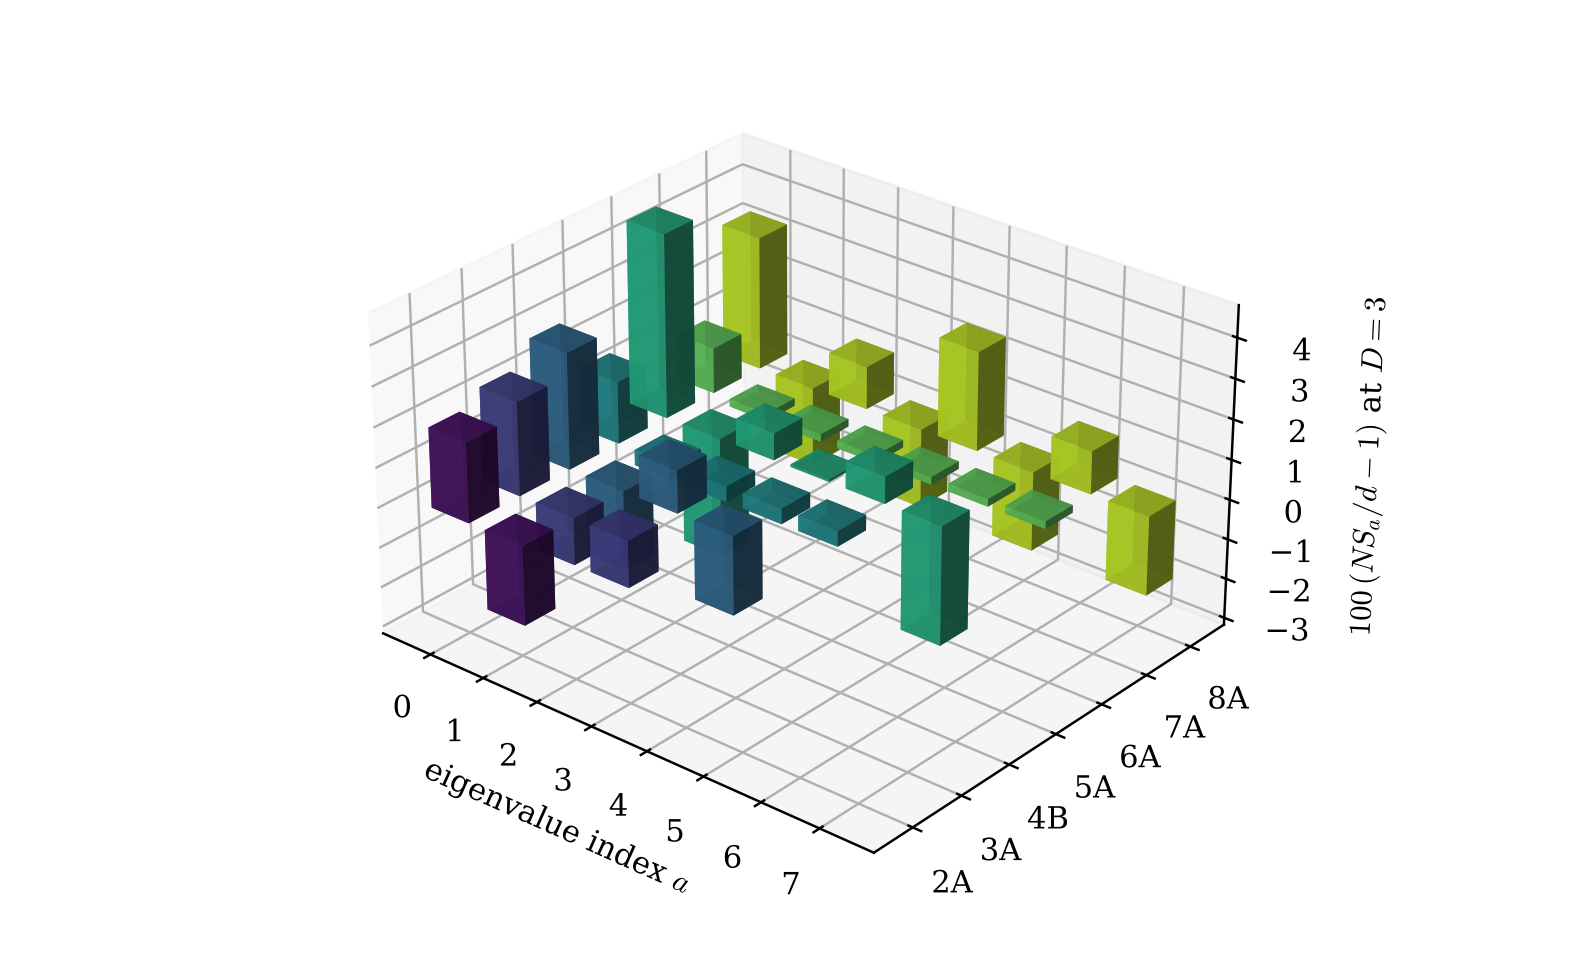
\includegraphics[width=0.85\textwidth]{figures/fig_sectors.png}
\caption{Deviation of the discrete information from equidistribution at the smallest discriminant $D=3$: the bars show $100\,(N S_a/d-1)$ for each type and each eigenvalue $e^{2\pi ia/N}$. All values lie between $-3.1$ and $+4.7$ per cent; at $D=7$ their absolute values are below $1.1$ per cent.}
\label{fig:sectors}
\end{figure}

\begin{figure}[t]
\centering
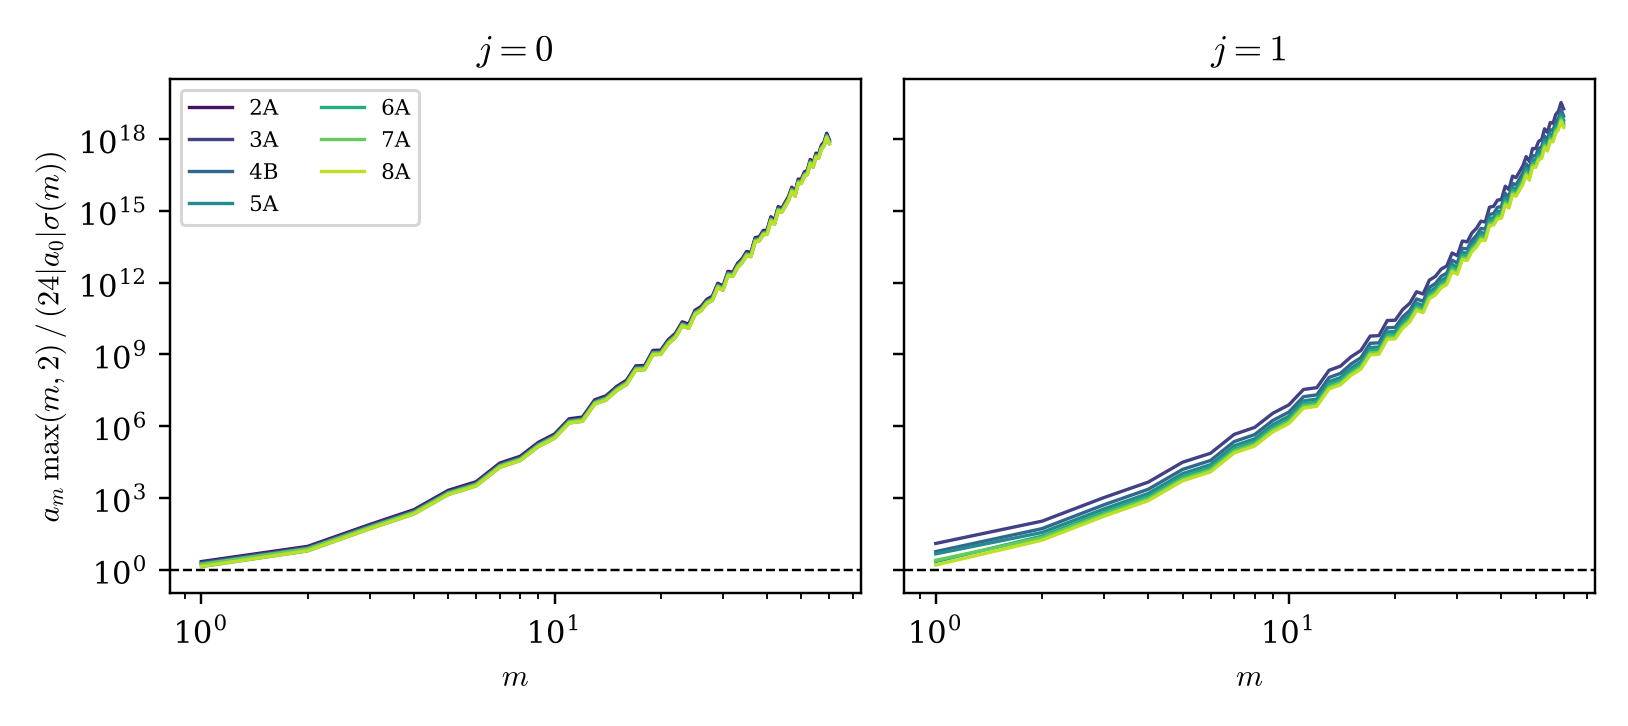
\includegraphics[width=0.95\textwidth]{figures/fig_margins.png}
\caption{The ratio $a_m\max(m,2)/(24|a_0|\sigma(m))$ for the series $k_0$ (left) and $k_1$ (right), $1\le m\le60$. Condition \eqref{eq:cond} requires the ratio to exceed one (dashed line). For $2A$ and $\mu=1$ one has $a_0=0$ and the curve is omitted.}
\label{fig:margins}
\end{figure}

\section{Discussion}\label{sec:discussion}

To our knowledge, Theorem~\ref{thm:A} is the first proof of the positivity of discrete information for an infinite family of charges. Three features of the proof are worth isolating. First, Lemma~\ref{lem:strip} and Theorem~\ref{thm:finite} show that for magnetic charge one Sen's attractor contour for twined indices is equivalent to taking the Fourier coefficients of a single mock Jacobi form, uniformly in the twining. Second, Theorem~\ref{thm:B} identifies this mock Jacobi form explicitly: the twining changes the holomorphic part $f_gA+h_gB$ and the eta quotient, while the mock part is always a multiple of the class number generating function $\cH$, with coefficient $-2d_g(2)$ fixed by the residue at $z=0$. Third, the twined indices are dominated by the untwined one at every charge, not only asymptotically.

For magnetic charge $P^2=4$ the polar part is again a multiple of an Appell--Lerch sum, and the decomposition of \cite{BM13} for index two should allow the same argument; we have not carried it out. For larger magnetic charge the polar part has several components and the finite part is no longer determined by the residue at $z=0$ alone; there the comparison of Theorem~\ref{thm:C} would require bounds for the coefficients of the mock Jacobi forms $\psi^F_{g,m}$ of general index. Twisted-twining partition functions of the CHL orbifolds \cite{GSSV23} and torsion larger than one are also not covered by our results.

\appendix

\section{The twining genus from the fixed points}\label{app:genus}

Let $g$ act on $X$ with isolated fixed points $x_1,\dots,x_{\chi_g}$, and at $x_j$ by $\operatorname{diag}(\zeta_j,\zeta_j^{-1})$, $\zeta_j=e^{2\pi i\alpha_j}$. By the holomorphic Lefschetz formula applied to the twisted Dolbeault complexes that define the elliptic genus, the $g$-equivariant elliptic genus localises to the fixed points \cite{BL00,HBJ92}:
\[
\phi_g(\tau,z)=\sum_{j=1}^{\chi_g}\prod_{\epsilon=\pm1}\frac{\vt_1(\tau,z+\epsilon\alpha_j)}{\vt_1(\tau,\epsilon\alpha_j)}=-\sum_{j=1}^{\chi_g}\frac{\vt_1(\tau,z+\alpha_j)\,\vt_1(\tau,z-\alpha_j)}{\vt_1(\tau,\alpha_j)^2},
\]
where $\vt_1(\tau,z)=-iq^{1/8}(y^{1/2}-y^{-1/2})\prod_{n\ge1}(1-q^n)(1-q^ny)(1-q^ny^{-1})$. Each local term equals $1$ at $z=0$, so $\phi_g(\tau,0)=\chi_g$. Using the product formula, with $c=\zeta+\zeta^{-1}=2\cos2\pi\alpha$,
\begin{equation}\label{eq:local}
-\frac{\vt_1(\tau,z+\alpha)\vt_1(\tau,z-\alpha)}{\vt_1(\tau,\alpha)^2}=\frac{y+y^{-1}-c}{2-c}\prod_{n\ge1}\frac{(1-cq^ny+q^{2n}y^2)(1-cq^ny^{-1}+q^{2n}y^{-2})}{(1-cq^n+q^{2n})^2}.
\end{equation}
Indeed $(y^{1/2}\zeta^{1/2}-y^{-1/2}\zeta^{-1/2})(y^{1/2}\zeta^{-1/2}-y^{-1/2}\zeta^{1/2})=y+y^{-1}-c$, $(\zeta^{1/2}-\zeta^{-1/2})^2=c-2$, and $(1-q^ny\zeta)(1-q^ny\zeta^{-1})=1-cq^ny+q^{2n}y^2$.

\begin{proof}[Proof of Proposition~\ref{prop:genus}]
Since $\phi_g$ is a weak Jacobi form of weight $0$ and index one for $\Gamma_0(N)$, even in $z$, Lemma~\ref{lem:structure} gives $\phi_g=\frac{\phi_g(\tau,0)}{12}B+T\,A$ with $T\in M_2(\Gamma_0(N))$, and $\phi_g(\tau,0)=\chi_g$. The space $M_2(\Gamma_0(N))$ has dimension at most $3$ for $N\le8$, and Sturm's bound for weight two on $\Gamma_0(N)$ is $\frac{2}{12}N\prod_{p\mid N}(1+\frac1p)\le2$. The coefficients of $\phi_g$ computed from \eqref{eq:local} in the cyclotomic field $\QQ(e^{2\pi i/N})$ agree exactly with those of $\frac{\chi_g}{12}B+T_gA$ for all exponents of $q$ up to $20$, far beyond this bound. Hence $T=T_g$.
\end{proof}

\section{Exact values and constants}\label{app:tables}

\begin{table}[H]
\centering
\caption{The twined single-centred indices $d_g(D)$ for the smallest discriminants. For $2A$, $3A$ and $4B$ they agree with the entries $-B_6^{g}$ of Tables~3, 6 and~9 of \cite{GSSV23} at $(Q^2,P^2)=(2,2),(2,4),(2,6)$ and $Q\cdot P\in\{0,1\}$, the tables being symmetric under $Q^2\leftrightarrow P^2$.}
\label{tab:values}
\renewcommand{\arraystretch}{1.15}
\begin{tabular}{crrrrrr}
\toprule
$g$ & $D=3$ & $D=4$ & $D=7$ & $D=8$ & $D=11$ & $D=12$\\
\midrule
$1A$ & 25353 & 50064 & 561576 & 1127472 & 8533821 & 16491600\\
$2A$ & 505 & $-1328$ & 3128 & $-7696$ & 14781 & $-33520$\\
$3A$ & 297 & $-588$ & 1272 & $-2442$ & 4998 & $-8964$\\
$4B$ & 117 & $-224$ & 444 & $-768$ & 1437 & $-2400$\\
$5A$ & 98 & $-176$ & 336 & $-588$ & 1056 & $-1680$\\
$6A$ & 37 & $-44$ & 80 & $-130$ & 246 & $-340$\\
$7A$ & 48 & $-84$ & 141 & $-228$ & 387 & $-582$\\
$8A$ & 27 & $-40$ & 54 & $-96$ & 165 & $-224$\\
\bottomrule
\end{tabular}
\end{table}

\begin{table}[H]
\centering
\caption{Constants of Section~\ref{sec:proofC}: the sums $c_A$, $c_B$, $H_\Sigma$ over the nontrivial powers of $g$, the constant terms $a_0$ of $k_0$ and $k_1$, and the points $m_0$ from which the analytic bound of Corollary~\ref{cor:large} holds.}
\label{tab:consts}
\renewcommand{\arraystretch}{1.15}
\begin{tabular}{crrrrrrr}
\toprule
$g$ & $c_A$ & $c_B$ & $H_\Sigma$ & $a_0(k_0)$ & $a_0(k_1)$ & $m_0(k_0)$ & $m_0(k_1)$\\
\midrule
$2A$ & $1.889$ & $1.111$ & 104 & $-64$ & $0$ & 1089 & 1720\\
$3A$ & $3.750$ & $2.250$ & 108 & $-72$ & $-3$ & 1720 & 2719\\
$4B$ & $7.244$ & $3.222$ & 168 & $-80$ & $-6$ & 2483 & 3929\\
$5A$ & $25.472$ & $3.889$ & 112 & $-80$ & $-9$ & 4914 & 7784\\
$6A$ & $16.336$ & $5.222$ & 240 & $-96$ & $-12$ & 4005 & 6343\\
$7A$ & $42.763$ & $5.250$ & 108 & $-84$ & $-15$ & 6810 & 10792\\
$8A$ & $20.511$ & $6.444$ & 216 & $-96$ & $-18$ & 4645 & 7356\\
\bottomrule
\end{tabular}
\end{table}

\section{Computations}\label{app:code}

Three finite computations enter the proofs, all in exact rational arithmetic with the FLINT library: (i) the coefficients of $\phi_g$ in Proposition~\ref{prop:genus} up to $q^{20}$, in exact arithmetic in $\QQ(e^{2\pi i/N})$; (ii) the expansions of $f$ and $h$ in Theorem~\ref{thm:B} from \eqref{eq:X2} and \eqref{eq:moments}, compared with Table~\ref{tab:fh} up to the Sturm bound $q^{129}$ for $\Gamma(4N)$; (iii) the coefficients $a_m$ of the fourteen series $k_\mu$ for $m\le12045$ and condition \eqref{eq:cond}. The class numbers are computed by counting reduced forms. The identity of Proposition~\ref{prop:DMZ} was checked in the same way up to $q^{99}$. As an independent check, $S_a$ was computed for all $D\le600$ and every type from the theta components of Theorem~\ref{thm:B}; every $S_a$ is a positive integer, and the values for $N=2,3,4$ agree with \cite{GSSV23}. The programs and their output are archived at \cite{Bha26}.

\FloatBarrier
\section*{Declarations}
\noindent\textbf{Data availability.} The programs that carry out the computations of Appendix~\ref{app:code} and their output are available in the archive \cite{Bha26}.

\noindent\textbf{Funding.} This research received no external funding.

\noindent\textbf{Conflicts of interest.} The author declares no conflict of interest.

\noindent\textbf{Ethics.} Not applicable; this work involves no human or animal subjects.

\begingroup\raggedright
\begin{thebibliography}{99}
\bibitem{And84} G.~E.~Andrews, \emph{The Theory of Partitions}, Cambridge University Press, Cambridge, 1984. doi:10.1017/CBO9780511608650

\bibitem{BBS23} D.~Bhattacharjee, P.~Bose, P.~Samal, \emph{Ramanujan $\tau$-function and its relationship with $PSL(2,\mathbb Z)$ for $\mathcal L_{24}(\tau)^{+,E}$}, Research Square (2023). doi:10.21203/rs.3.rs-2796280/v1

\bibitem{Bha22} D.~Bhattacharjee, \emph{Generalization of quartic and quintic Calabi--Yau manifolds fibered by polarized K3 surfaces}, Research Square (2022). doi:10.21203/rs.3.rs-1965255/v1

\bibitem{Bha26} D.~Bhattacharjee, \emph{Code and data for: Black holes carry positive discrete information}, version v1.0.0, Zenodo (2026). doi:\zenodoDOI

\bibitem{BL00} L.~Borisov, A.~Libgober, \emph{Elliptic genera of toric varieties and applications to mirror symmetry}, Invent. Math. \textbf{140} (2000), 453--485. doi:10.1007/s002220000058

\bibitem{BM13} K.~Bringmann, S.~Murthy, \emph{On the positivity of black hole degeneracies in string theory}, Commun. Number Theory Phys. \textbf{7} (2013), 15--56. doi:10.4310/CNTP.2013.v7.n1.a2

\bibitem{BN26} D.~Bhattacharjee, P.~Nandi, \emph{Enriques and Kummer surfaces arising from K3 involutions}, Preprints (2026). doi:10.20944/preprints202602.0098.v1

\bibitem{BSS09} S.~Banerjee, A.~Sen, Y.~K.~Srivastava, \emph{Genus two surface and quarter BPS dyons: the contour prescription}, J. High Energy Phys. \textbf{2009}, no.~3 (2009), 151. doi:10.1088/1126-6708/2009/03/151

\bibitem{CD21} A.~Chattopadhyaya, J.~R.~David, \emph{Horizon states and the sign of their index in $\mathcal N=4$ dyons}, J. High Energy Phys. \textbf{2021}, no.~3 (2021), 106. doi:10.1007/JHEP03(2021)106

\bibitem{Che10} M.~C.~N.~Cheng, \emph{K3 surfaces, $\mathcal N=4$ dyons and the Mathieu group $M_{24}$}, Commun. Number Theory Phys. \textbf{4} (2010), 623--657. doi:10.4310/CNTP.2010.v4.n4.a2

\bibitem{CV08} M.~C.~N.~Cheng, E.~P.~Verlinde, \emph{Wall crossing, discrete attractor flow and Borcherds algebra}, SIGMA \textbf{4} (2008), 068. doi:10.3842/SIGMA.2008.068

\bibitem{DGMS11} A.~Dabholkar, J.~Gomes, S.~Murthy, A.~Sen, \emph{Supersymmetric index from black hole entropy}, J. High Energy Phys. \textbf{2011}, no.~4 (2011), 034. doi:10.1007/JHEP04(2011)034

\bibitem{DJS07} J.~R.~David, D.~P.~Jatkar, A.~Sen, \emph{Dyon spectrum in generic $\mathcal N=4$ supersymmetric $\mathbb Z_N$ orbifolds}, J. High Energy Phys. \textbf{2007}, no.~1 (2007), 016. doi:10.1088/1126-6708/2007/01/016

\bibitem{DMVV97} R.~Dijkgraaf, G.~Moore, E.~Verlinde, H.~Verlinde, \emph{Elliptic genera of symmetric products and second quantized strings}, Commun. Math. Phys. \textbf{185} (1997), 197--209. doi:10.1007/s002200050087

\bibitem{DVV97} R.~Dijkgraaf, E.~Verlinde, H.~Verlinde, \emph{Counting dyons in $N=4$ string theory}, Nucl. Phys. B \textbf{484} (1997), 543--561. doi:10.1016/S0550-3213(96)00640-2

\bibitem{EOT11} T.~Eguchi, H.~Ooguri, Y.~Tachikawa, \emph{Notes on the K3 surface and the Mathieu group $M_{24}$}, Exp. Math. \textbf{20} (2011), 91--96. doi:10.1080/10586458.2011.544585

\bibitem{EZ85} M.~Eichler, D.~Zagier, \emph{The Theory of Jacobi Forms}, Progress in Mathematics \textbf{55}, Birkh\"auser, Boston, 1985. doi:10.1007/978-1-4684-9162-3

\bibitem{Gan16} T.~Gannon, \emph{Much ado about Mathieu}, Adv. Math. \textbf{301} (2016), 322--358. doi:10.1016/j.aim.2016.06.014

\bibitem{GHV10} M.~R.~Gaberdiel, S.~Hohenegger, R.~Volpato, \emph{Mathieu twining characters for K3}, J. High Energy Phys. \textbf{2010}, no.~9 (2010), 058. doi:10.1007/JHEP09(2010)058

\bibitem{GK10} S.~Govindarajan, K.~Gopala Krishna, \emph{BKM Lie superalgebras from dyon spectra in $\mathbb Z_N$ CHL orbifolds for composite $N$}, J. High Energy Phys. \textbf{2010}, no.~5 (2010), 014. doi:10.1007/JHEP05(2010)014

\bibitem{Gov11} S.~Govindarajan, \emph{BKM Lie superalgebras from counting twisted CHL dyons}, J. High Energy Phys. \textbf{2011}, no.~5 (2011), 089. doi:10.1007/JHEP05(2011)089

\bibitem{GSSV23} S.~Govindarajan, S.~Samanta, P.~Shanmugapriya, A.~Virmani, \emph{Positivity of discrete information for CHL black holes}, Nucl. Phys. B \textbf{987} (2023), 116095. doi:10.1016/j.nuclphysb.2023.116095

\bibitem{HBJ92} F.~Hirzebruch, T.~Berger, R.~Jung, \emph{Manifolds and Modular Forms}, Aspects of Mathematics \textbf{E20}, Vieweg, Braunschweig, 1992. doi:10.1007/978-3-663-14045-0

\bibitem{HZ76} F.~Hirzebruch, D.~Zagier, \emph{Intersection numbers of curves on Hilbert modular surfaces and modular forms of Nebentypus}, Invent. Math. \textbf{36} (1976), 57--113. doi:10.1007/BF01390005

\bibitem{Muk88} S.~Mukai, \emph{Finite groups of automorphisms of K3 surfaces and the Mathieu group}, Invent. Math. \textbf{94} (1988), 183--221. doi:10.1007/BF01394352

\bibitem{Nik79} V.~V.~Nikulin, \emph{Finite groups of automorphisms of K\"ahlerian $K3$ surfaces}, Tr. Mosk. Mat. Obs. \textbf{38} (1979), 75--137; English transl. in Trans. Moscow Math. Soc.

\bibitem{PV14} D.~Persson, R.~Volpato, \emph{Second quantized Mathieu moonshine}, Commun. Number Theory Phys. \textbf{8} (2014), 403--509. doi:10.4310/CNTP.2014.v8.n3.a2

\bibitem{Rau13} M.~Raum, \emph{$M_{24}$-twisted product expansions are Siegel modular forms}, Commun. Number Theory Phys. \textbf{7} (2013), 469--495. doi:10.4310/CNTP.2013.v7.n3.a3

\bibitem{SBBT26} R.~Sadhu, D.~Bhattacharjee, S.~Bhattacharya, S.~N.~Thakur, \emph{$E_8\times E_8$ heterotic gravity and M-theory}, SSRN (2026). doi:10.2139/ssrn.6326718

\bibitem{Sen07} A.~Sen, \emph{Walls of marginal stability and dyon spectrum in $\mathcal N=4$ supersymmetric string theories}, J. High Energy Phys. \textbf{2007}, no.~5 (2007), 039. doi:10.1088/1126-6708/2007/05/039

\bibitem{Sen08} A.~Sen, \emph{Black hole entropy function, attractors and precision counting of microstates}, Gen. Relativ. Gravit. \textbf{40} (2008), 2249--2431. doi:10.1007/s10714-008-0626-4

\bibitem{Sen10} A.~Sen, \emph{Discrete information from CHL black holes}, J. High Energy Phys. \textbf{2010}, no.~11 (2010), 138. doi:10.1007/JHEP11(2010)138

\bibitem{Sen11} A.~Sen, \emph{How do black holes predict the sign of the Fourier coefficients of Siegel modular forms?}, Gen. Relativ. Gravit. \textbf{43} (2011), 2171--2183. doi:10.1007/s10714-011-1175-9

\bibitem{Stu87} J.~Sturm, \emph{On the congruence of modular forms}, in: Number Theory (New York, 1984--1985), Lecture Notes in Math. \textbf{1240}, Springer, Berlin, 1987, 275--280. doi:10.1007/BFb0072985

\bibitem{Zag08} D.~Zagier, \emph{Elliptic modular forms and their applications}, in: The 1-2-3 of Modular Forms, Universitext, Springer, Berlin, 2008, 1--103. doi:10.1007/978-3-540-74119-0\_1
\end{thebibliography}
\endgroup

\end{document}
